\documentclass[a4paper]{article}
\usepackage[warn]{mathtext}
\usepackage[utf8]{inputenc}
\usepackage[T2A]{fontenc}
\usepackage[english,russian]{babel}
\usepackage{booktabs}
\usepackage{multicol}
\usepackage{fancyhdr}
\usepackage{graphicx}
\usepackage{microtype}
\usepackage{wrapfig}
\usepackage{amsmath}
\usepackage{floatflt}
\usepackage{geometry} \geometry{verbose,a4paper,tmargin=2cm,bmargin=2cm,lmargin=1.5cm,rmargin=1.5cm}
\usepackage{float}
\usepackage{amssymb}
\usepackage{caption}
\usepackage{epsfig}
\usepackage{newunicodechar}
\usepackage{color}

\begin{document}

\graphicspath{ {pictures/} }
\begin{center}
    {\scshape\Large Лабораторная работа по квантовой электронике} \par

    \

    {\huge\bfseries № 23 Инжекционные полупроводниковые лазеры} \par 

    \

    {\large Яромир Водзяновский Б04-855а}
\end{center}

\

\
\section{Введение}

    \subsection{Цель работы}
        
        \begin{enumerate}
            \item Измерение спектральных характеристик лазера и светодиодов, их дальнейший анализ
            \item Получение зависимости мощности излучения светодиодов и лазера от мощности накачки (Ватт-ваттаная характеристика)
        \end{enumerate}
        
    \subsection{Суть работы}
        \subsubsection{Спектральная характеристика}
            
        \begin{enumerate}
            \item Исследуем зависимось спеткра излучения инжекционного полупроводникового лазера/светодиодов от мощности накачки производится, измерив детектируемую длину волны и фиксируя напряжения при постоянной мощности накачки.
            \item Определим характер изменения формы спектральной характеристики от установленной мощности накачки для лазера.
        \end{enumerate}
            
        \subsubsection{Ватт-Ваттная характеристика}
        
            \begin{enumerate}
                \item Получим зависимости мощности излучения от мощности накачки для светодиодов и лазера поточечно меняя ток и напряжение накачки.
            \end{enumerate}
            
    
\section{Эксперимент}
    \subsection{Спектральные характеристики}
    
        \begin{enumerate}
            \item \textbf{Зависимость аплитуды излучения лазера от длины волны при разных токах накачки.} \par
        
                \begin{figure}[H]
                    \begin{center}
                        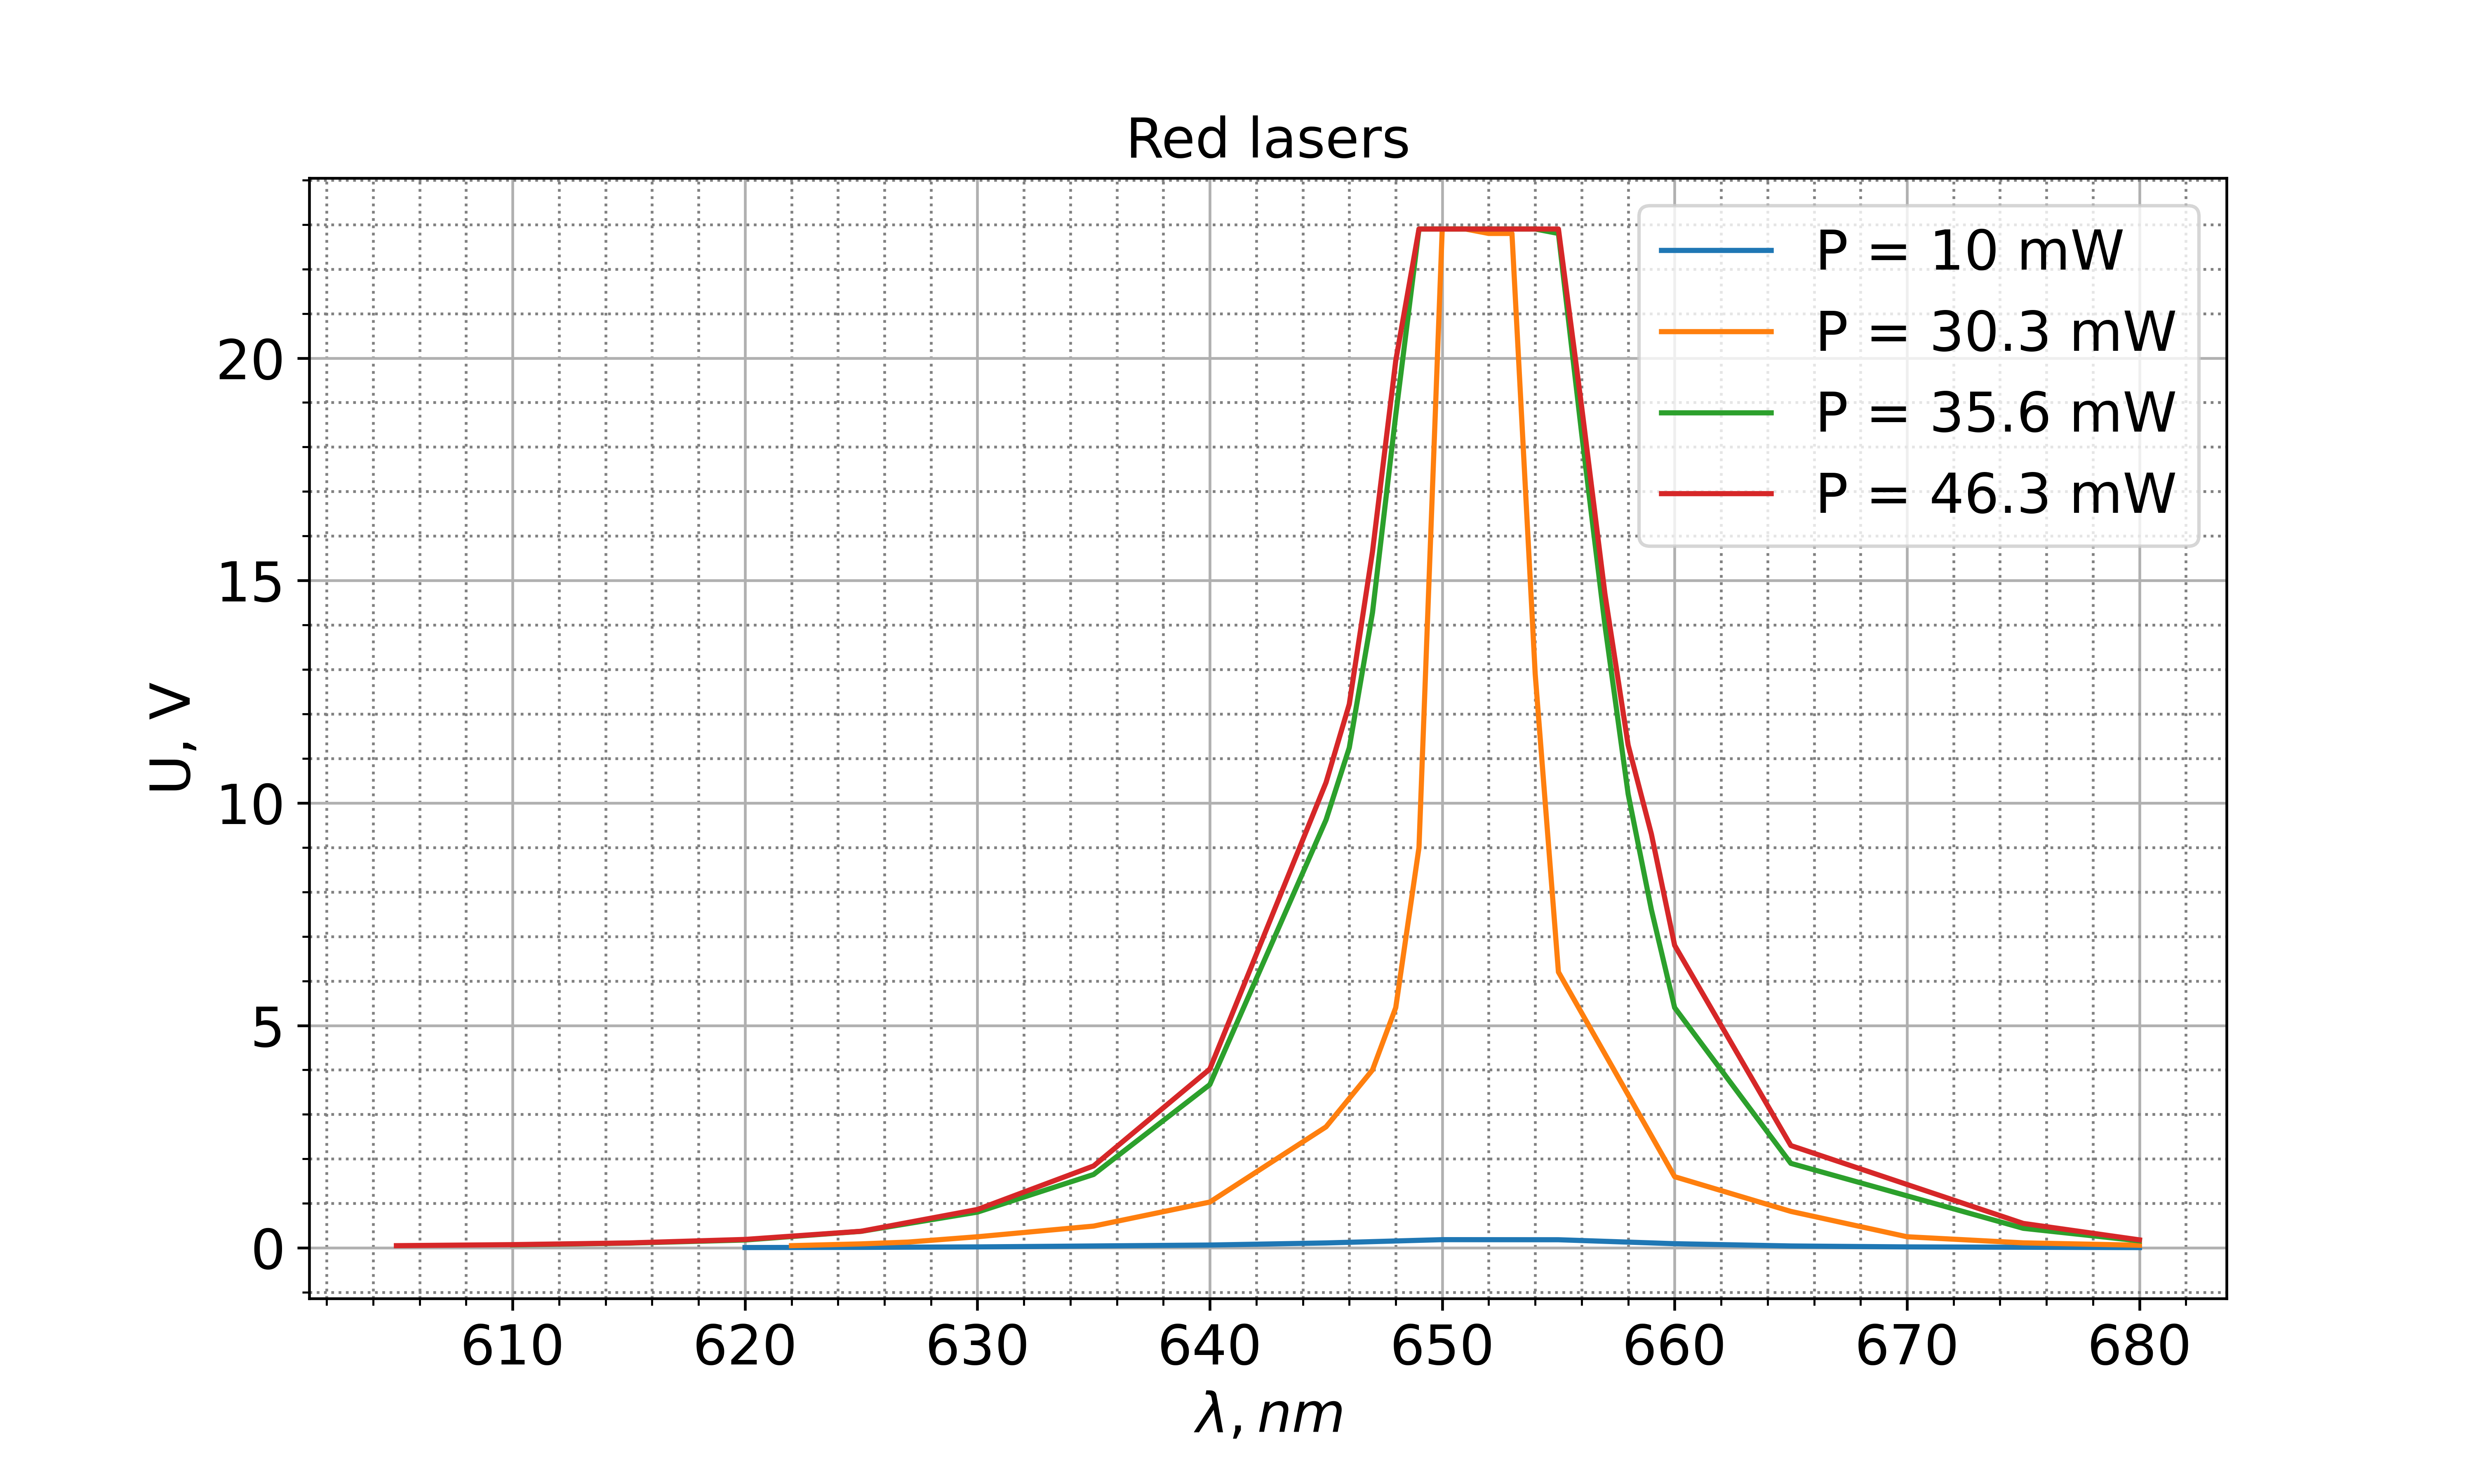
\includegraphics[scale=0.5]{spectr_red_lasers.png}
                        \caption{Характеристика лазера при разных мощностях накачки}
                        \label{lasers}
                    \end{center}
                \end{figure}
                
                При уменьшении накачки аплитуда выходного излучения падает, чем большн накачка - тем шире полосагенерации.
                
            \item \textbf{Зависимость аплитуды излучения диодов от длины волны при разных токах накачки.} \par
                
                \begin{figure}[H]
                    \begin{center}
                        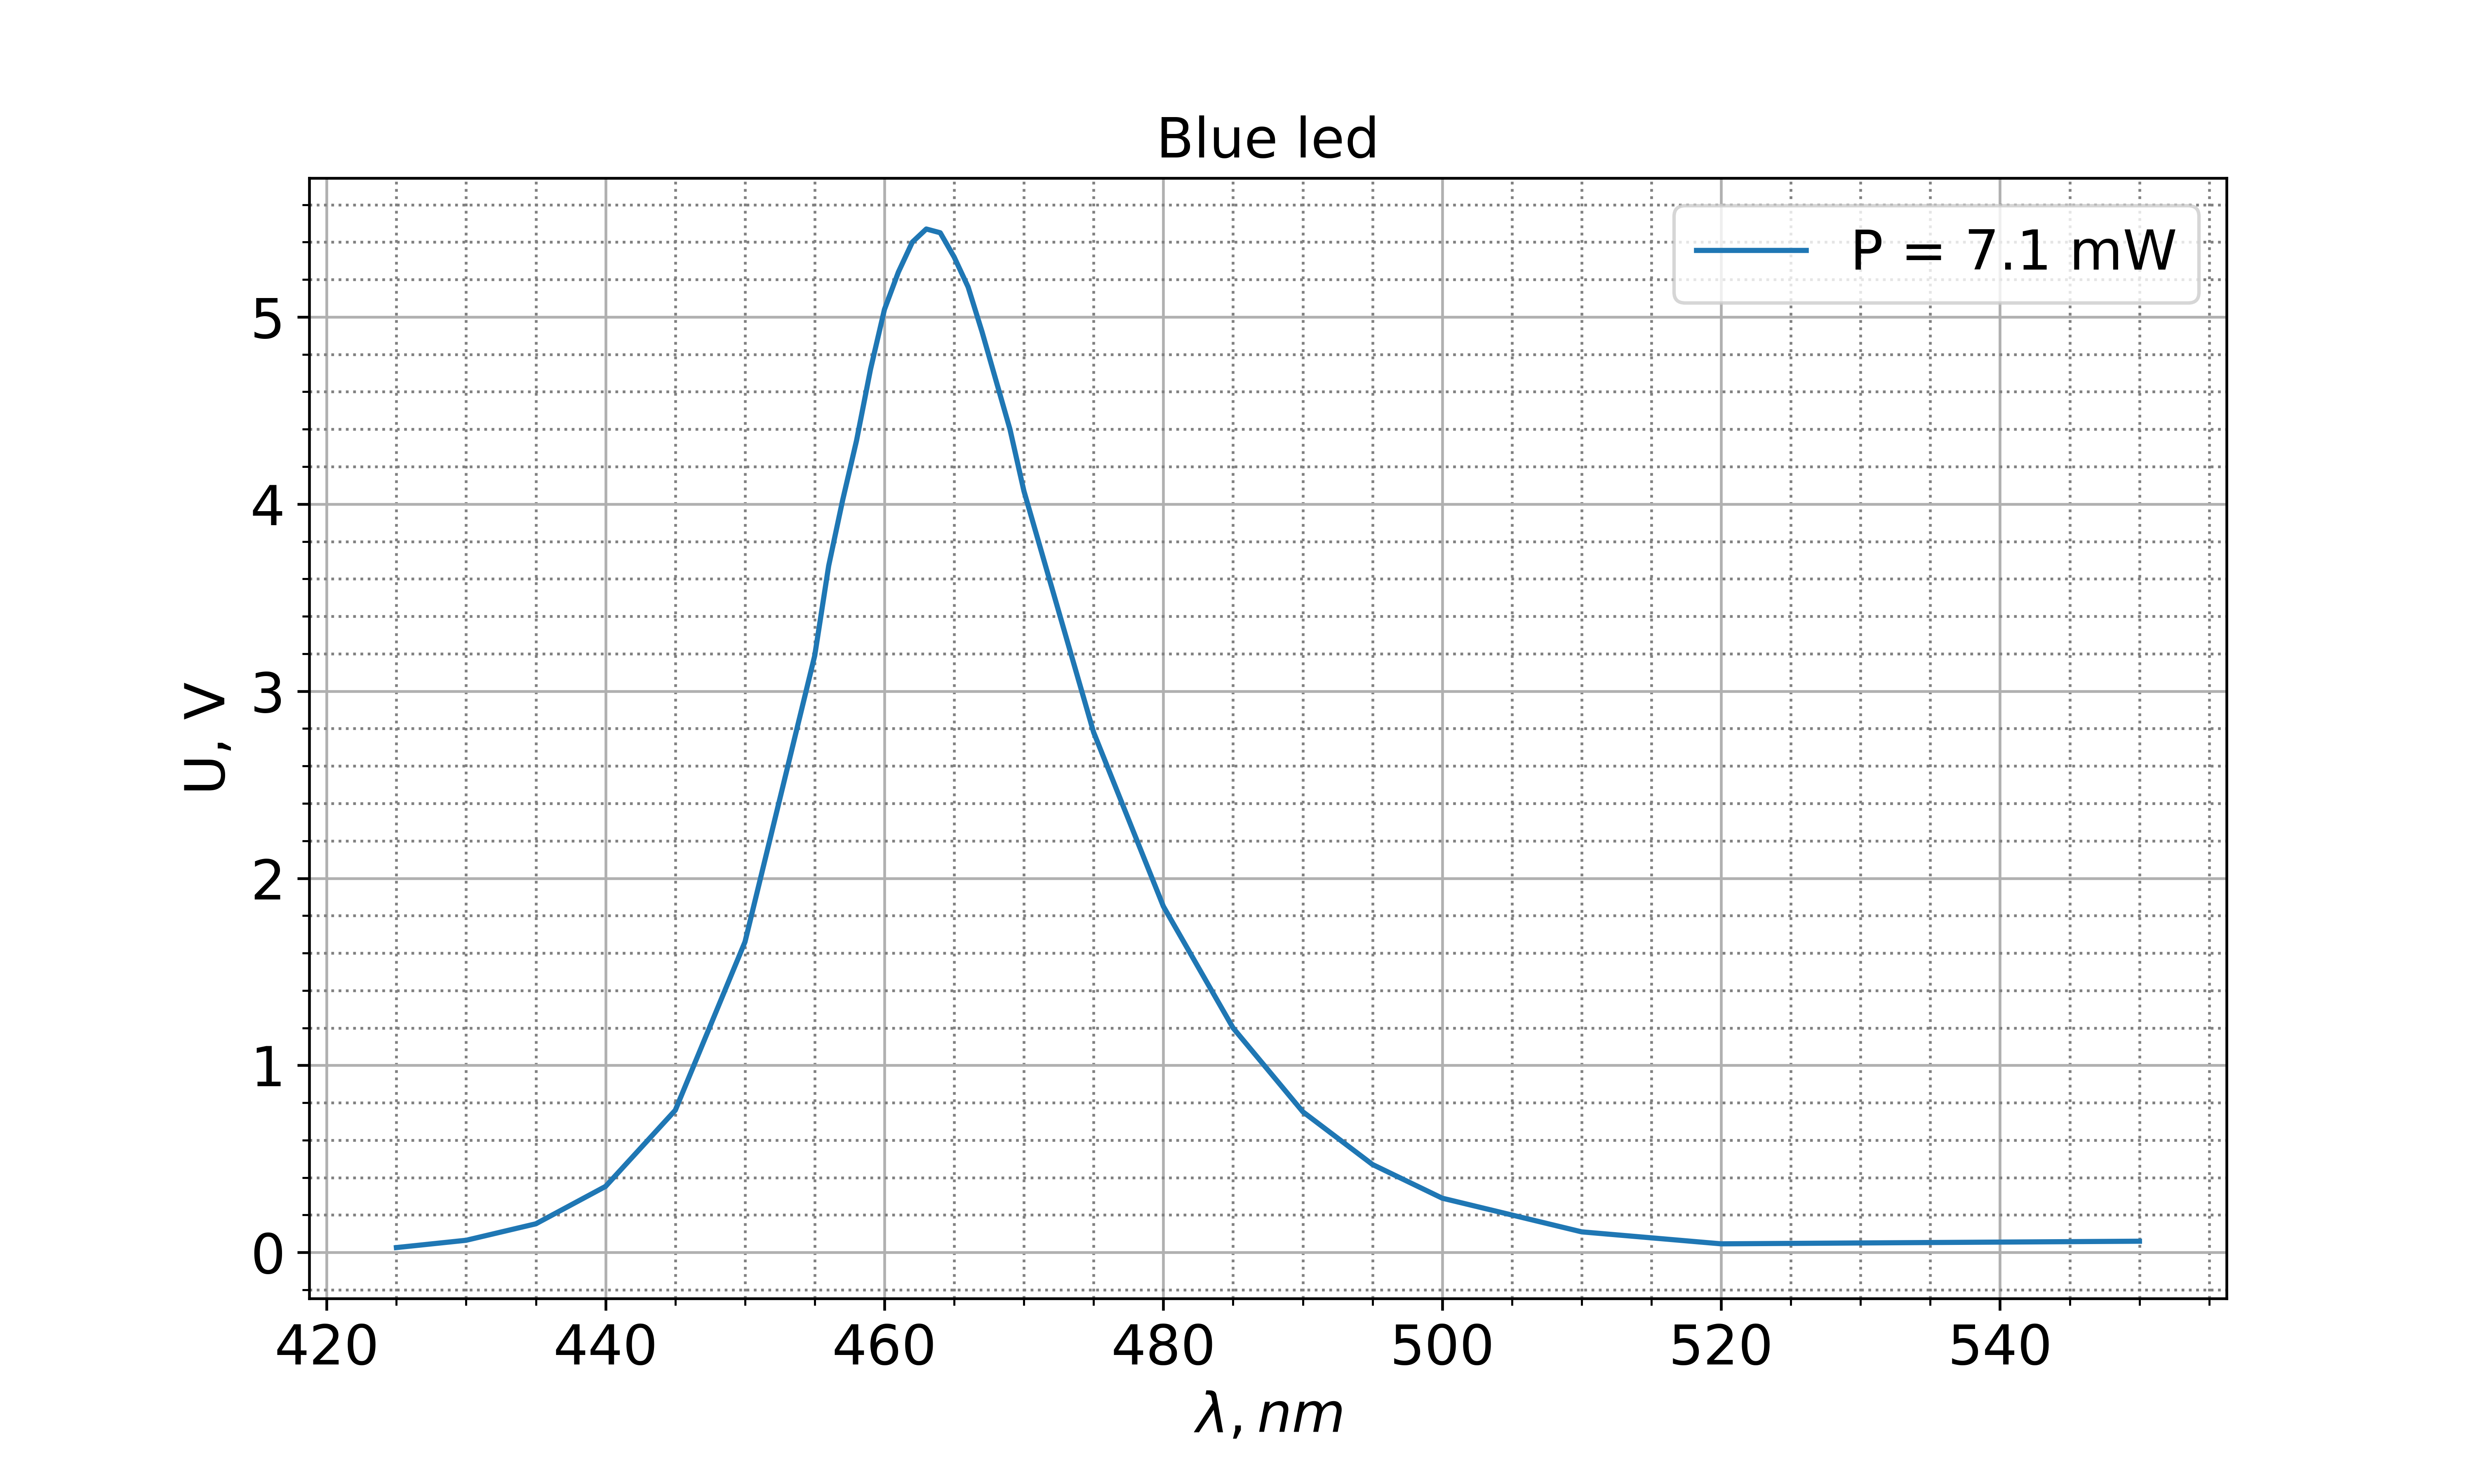
\includegraphics[scale=0.5]{spectr_blue_led.png}
                        \caption{Характеристика синего диода}
                        \label{blue}
                    \end{center}
                \end{figure}

                \begin{figure}[H]
                    \begin{center}
                        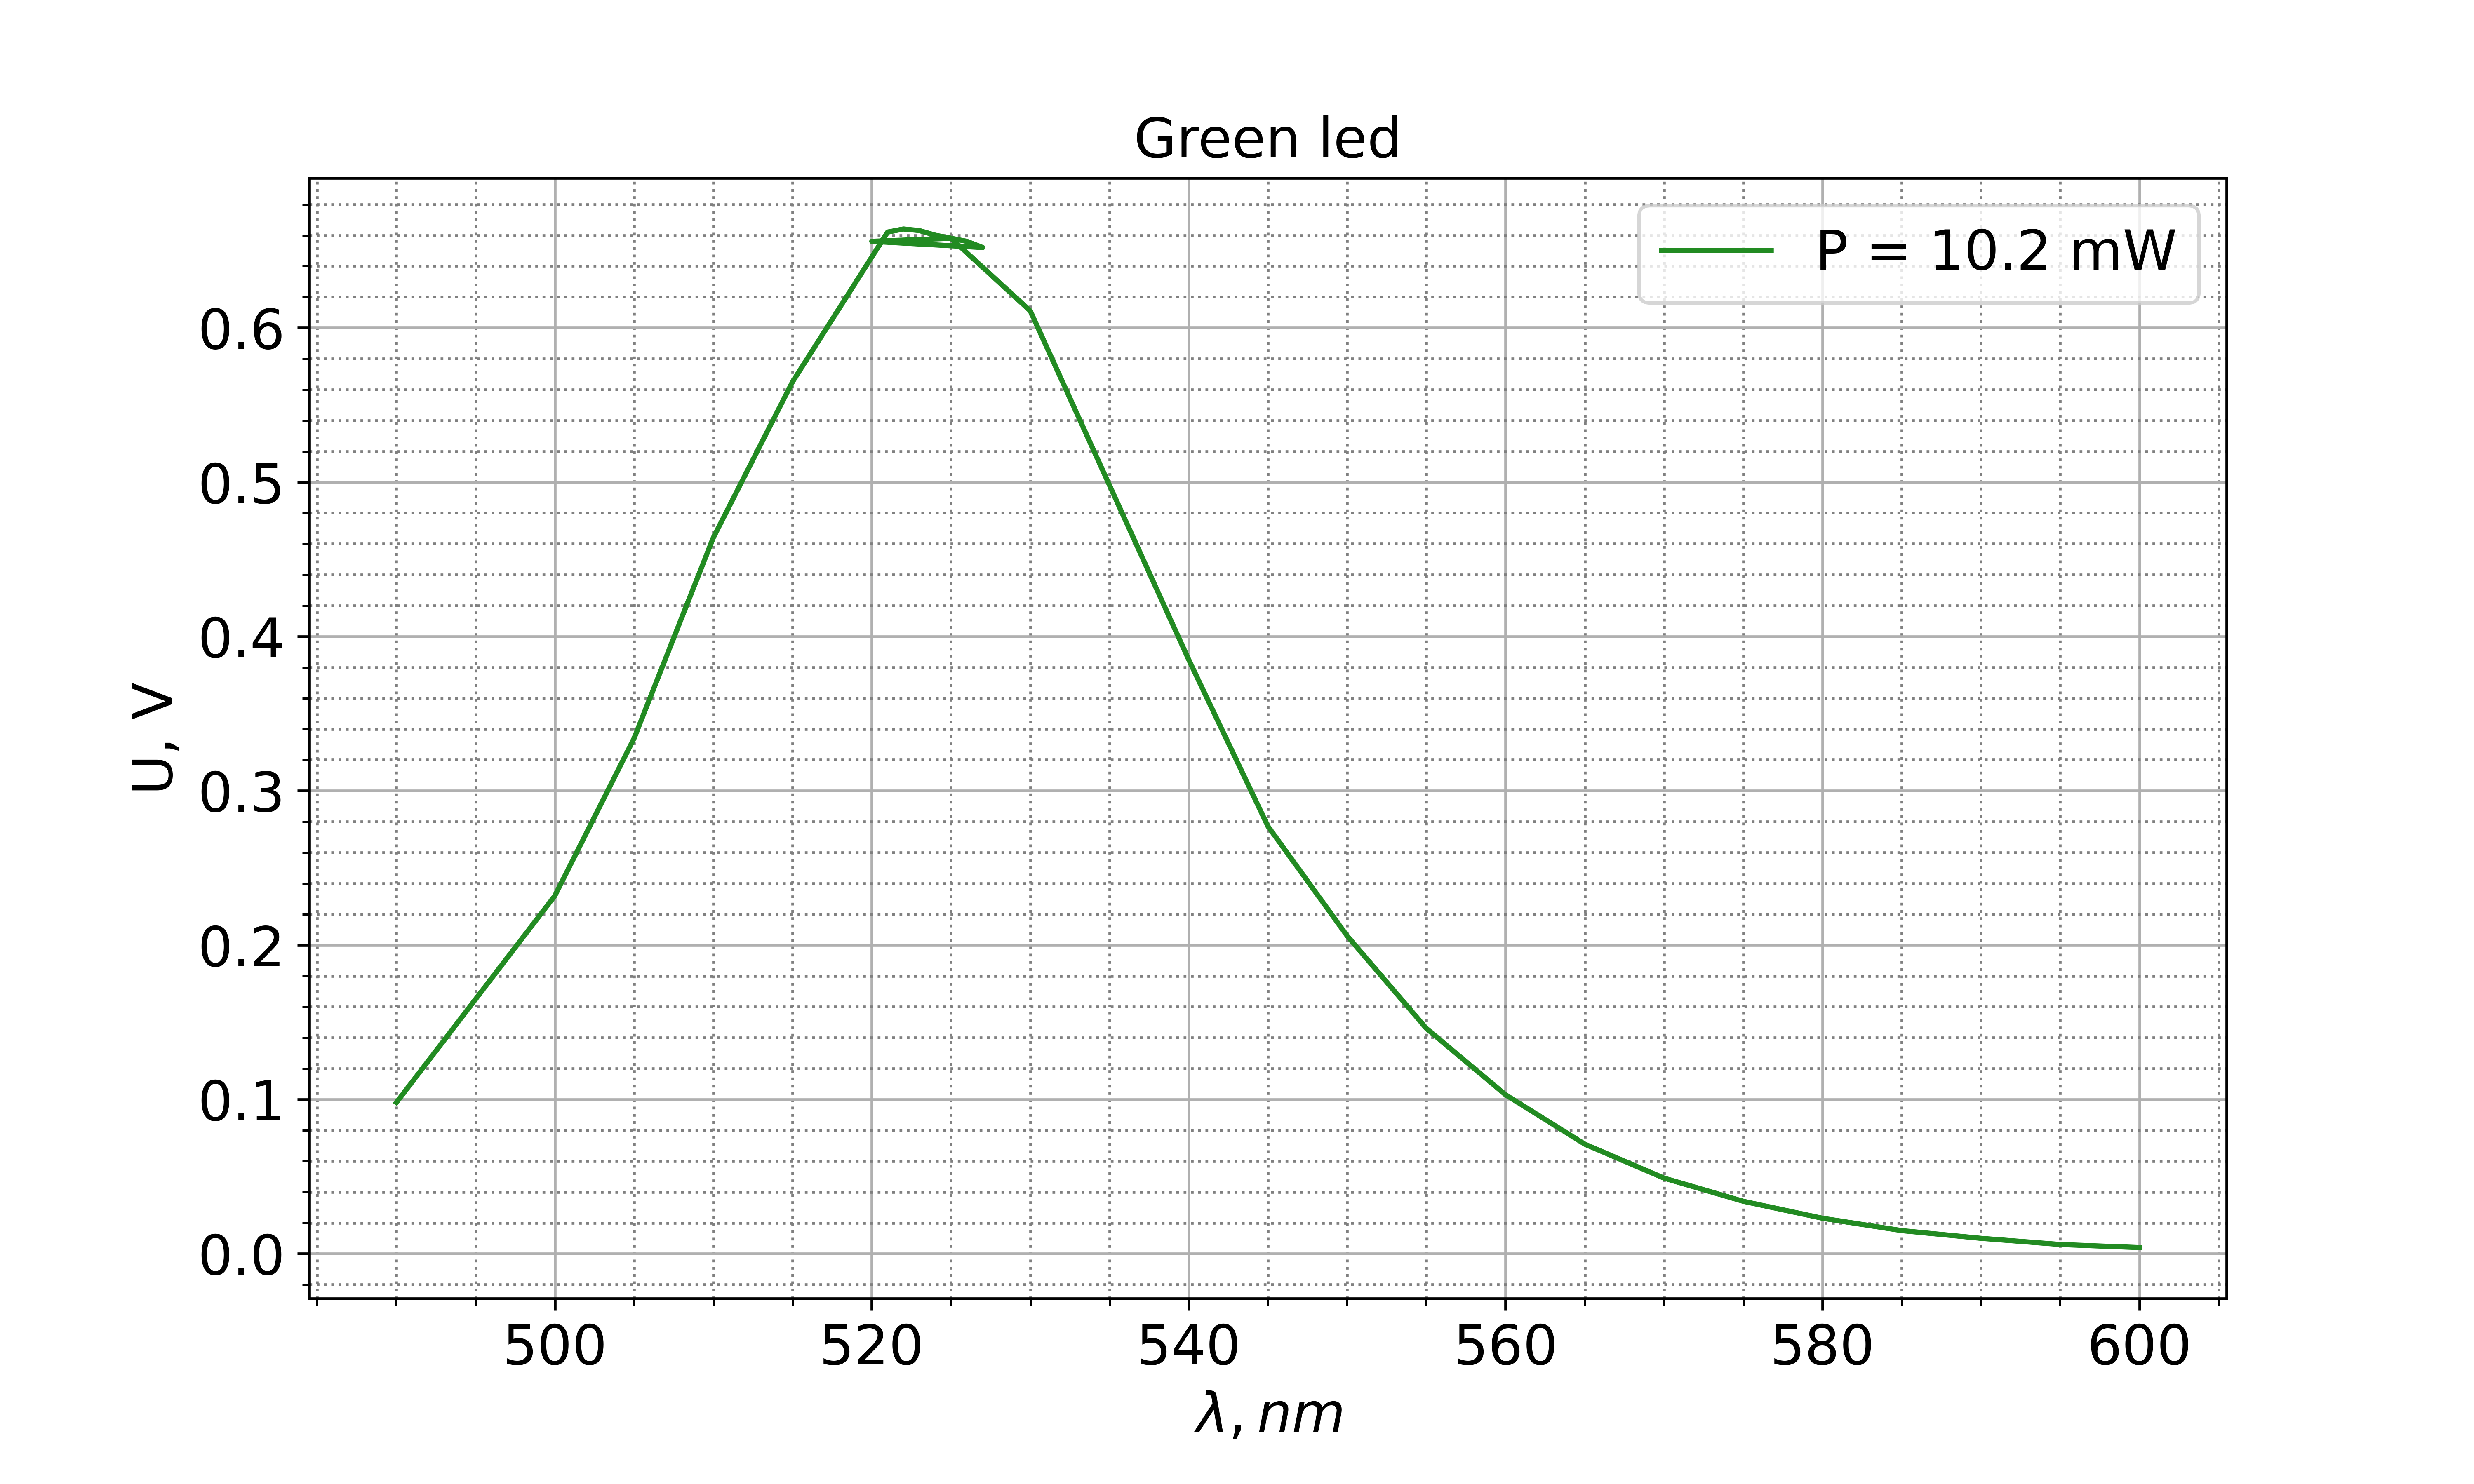
\includegraphics[scale=0.5]{spectr_green_led.png}
                        \caption{Характеристика зеленого диода}
                        \label{green}
                    \end{center}
                \end{figure}

                \begin{figure}[H]
                    \begin{center}
                        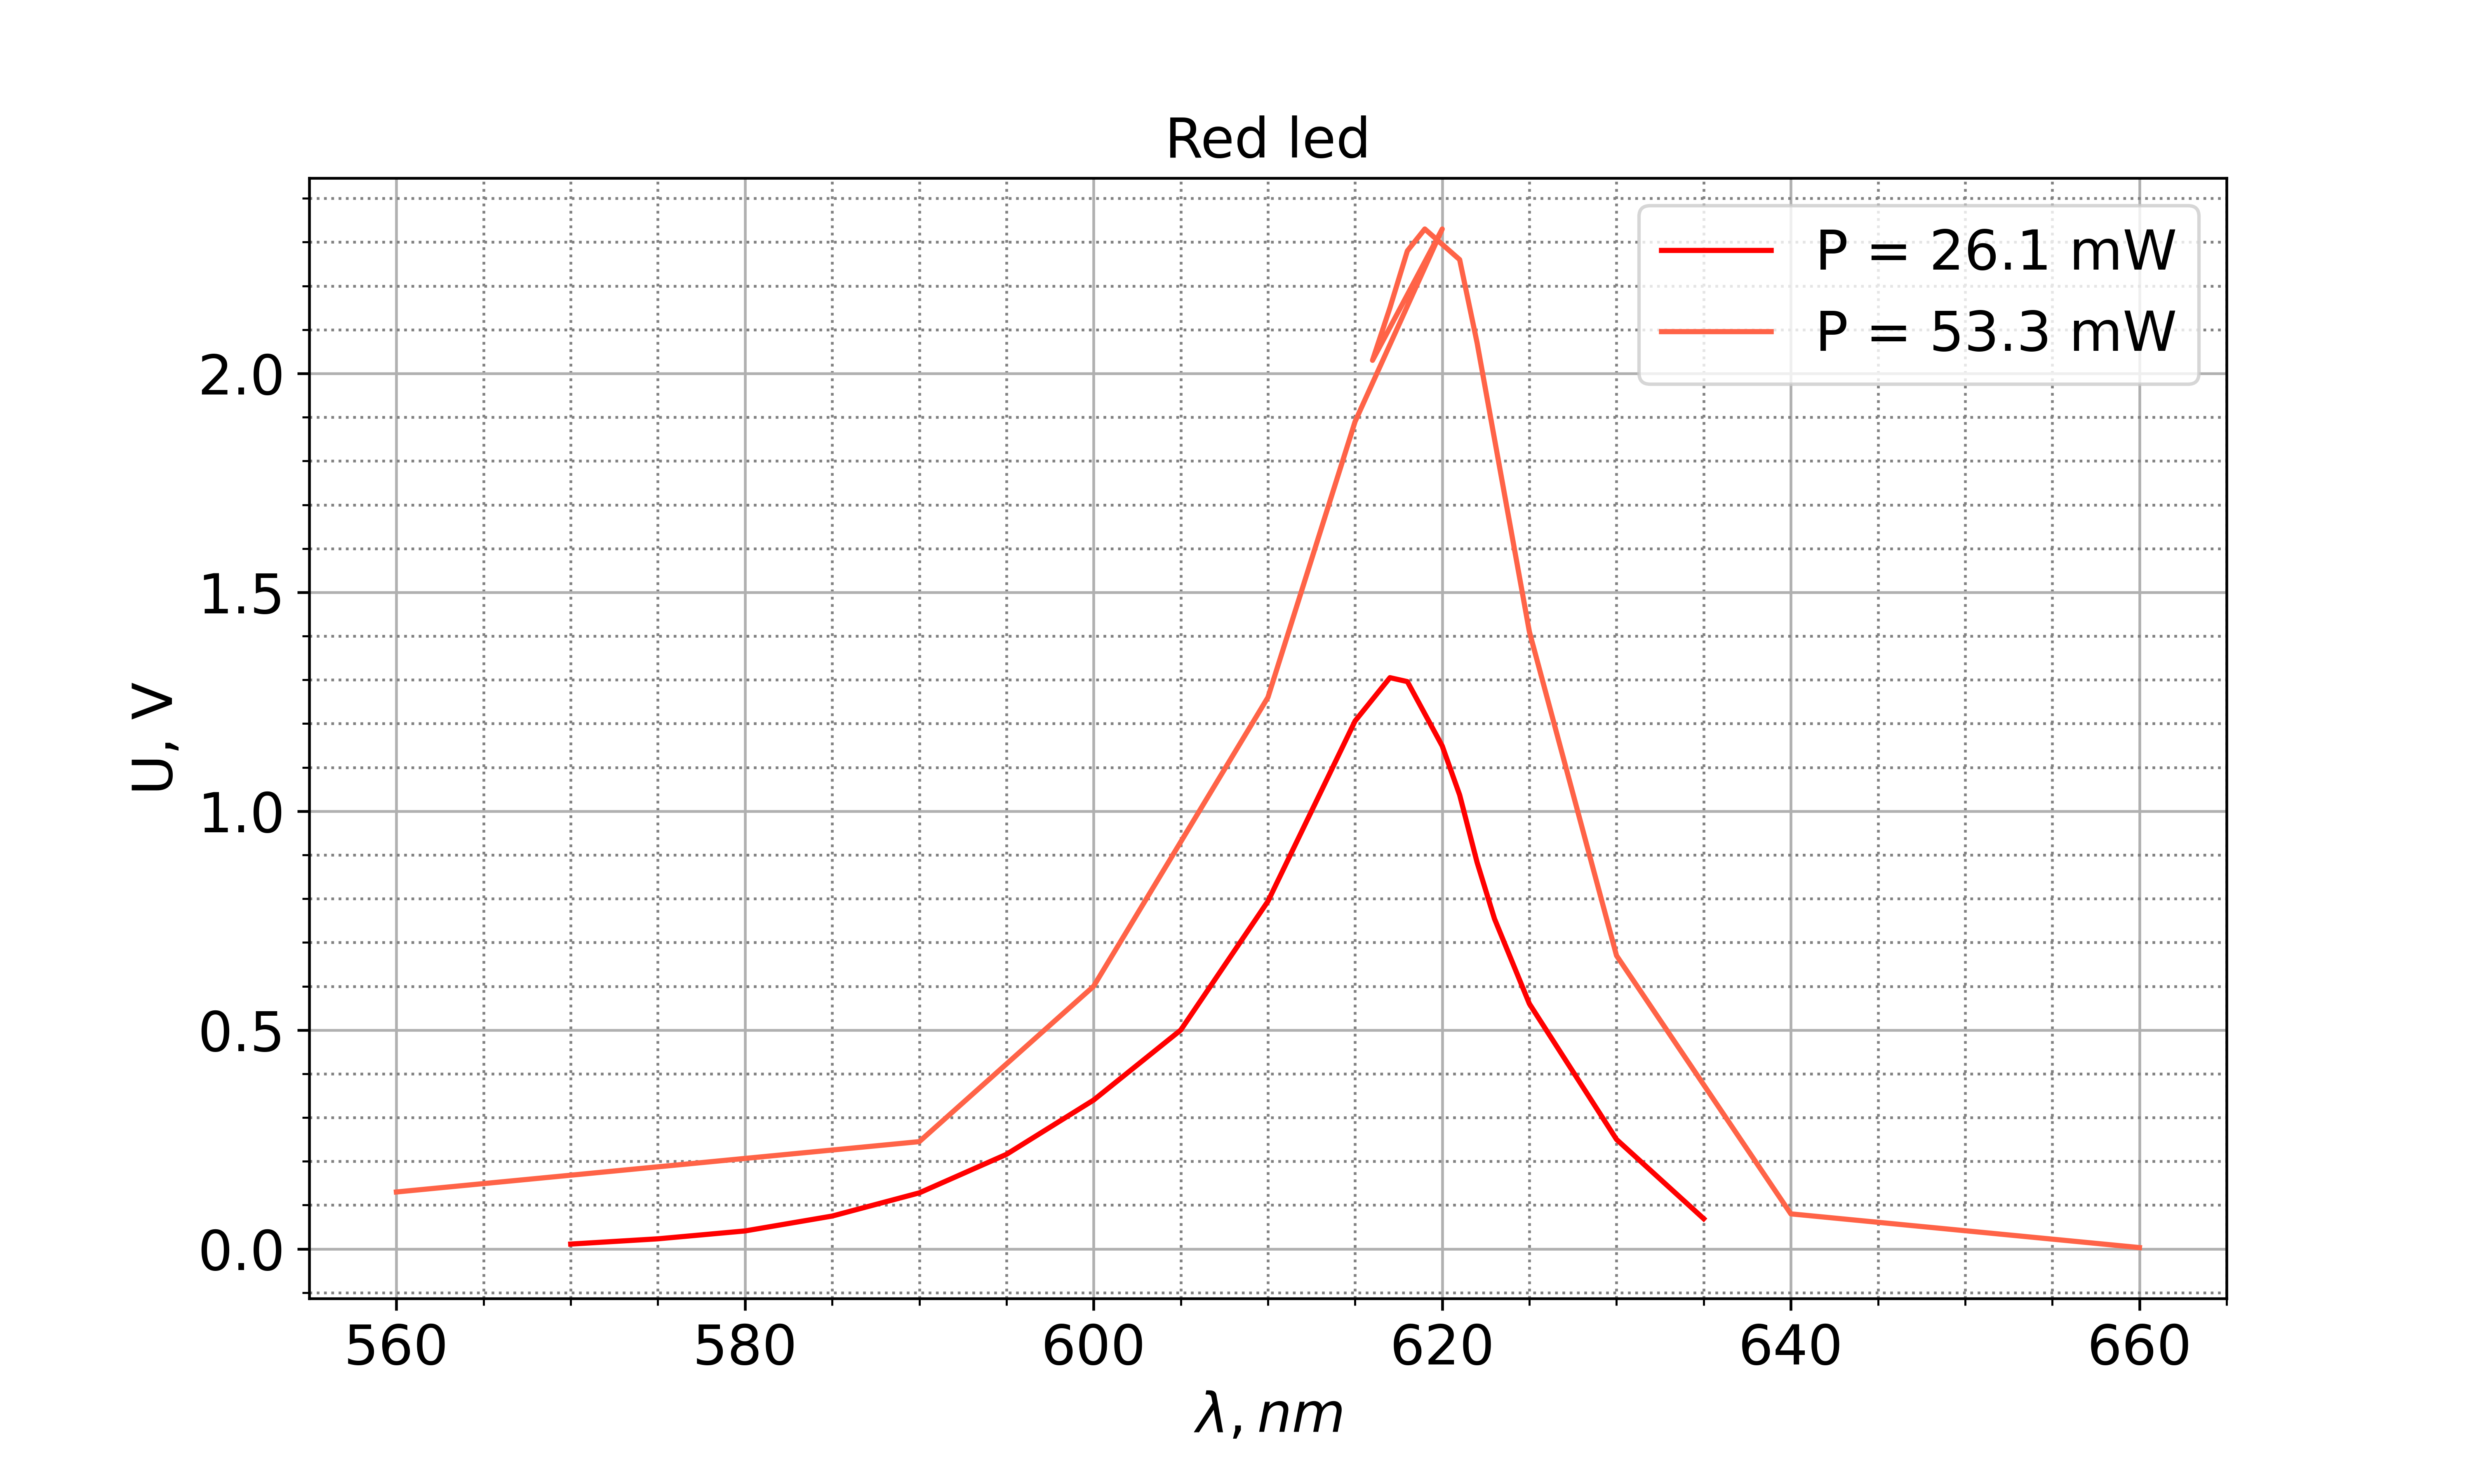
\includegraphics[scale=0.5]{spectr_red_led.png}
                        \caption{Характеристика красного диода}
                        \label{red}
                    \end{center}
                \end{figure}
                
                \par Соответсвующи приблизительные максимумы излучения: красный 617, зеленый 522, синий 462 nm.

	    \end{enumerate}

	\subsection{Ватт-ваттные характеристики}
	
        \begin{enumerate}
                
            \item \textbf{Зависимости амплитуды выходого сигнала от мощности накачки для двух лазеров} \par
            
                \begin{figure}[H]
                    \begin{center}
                        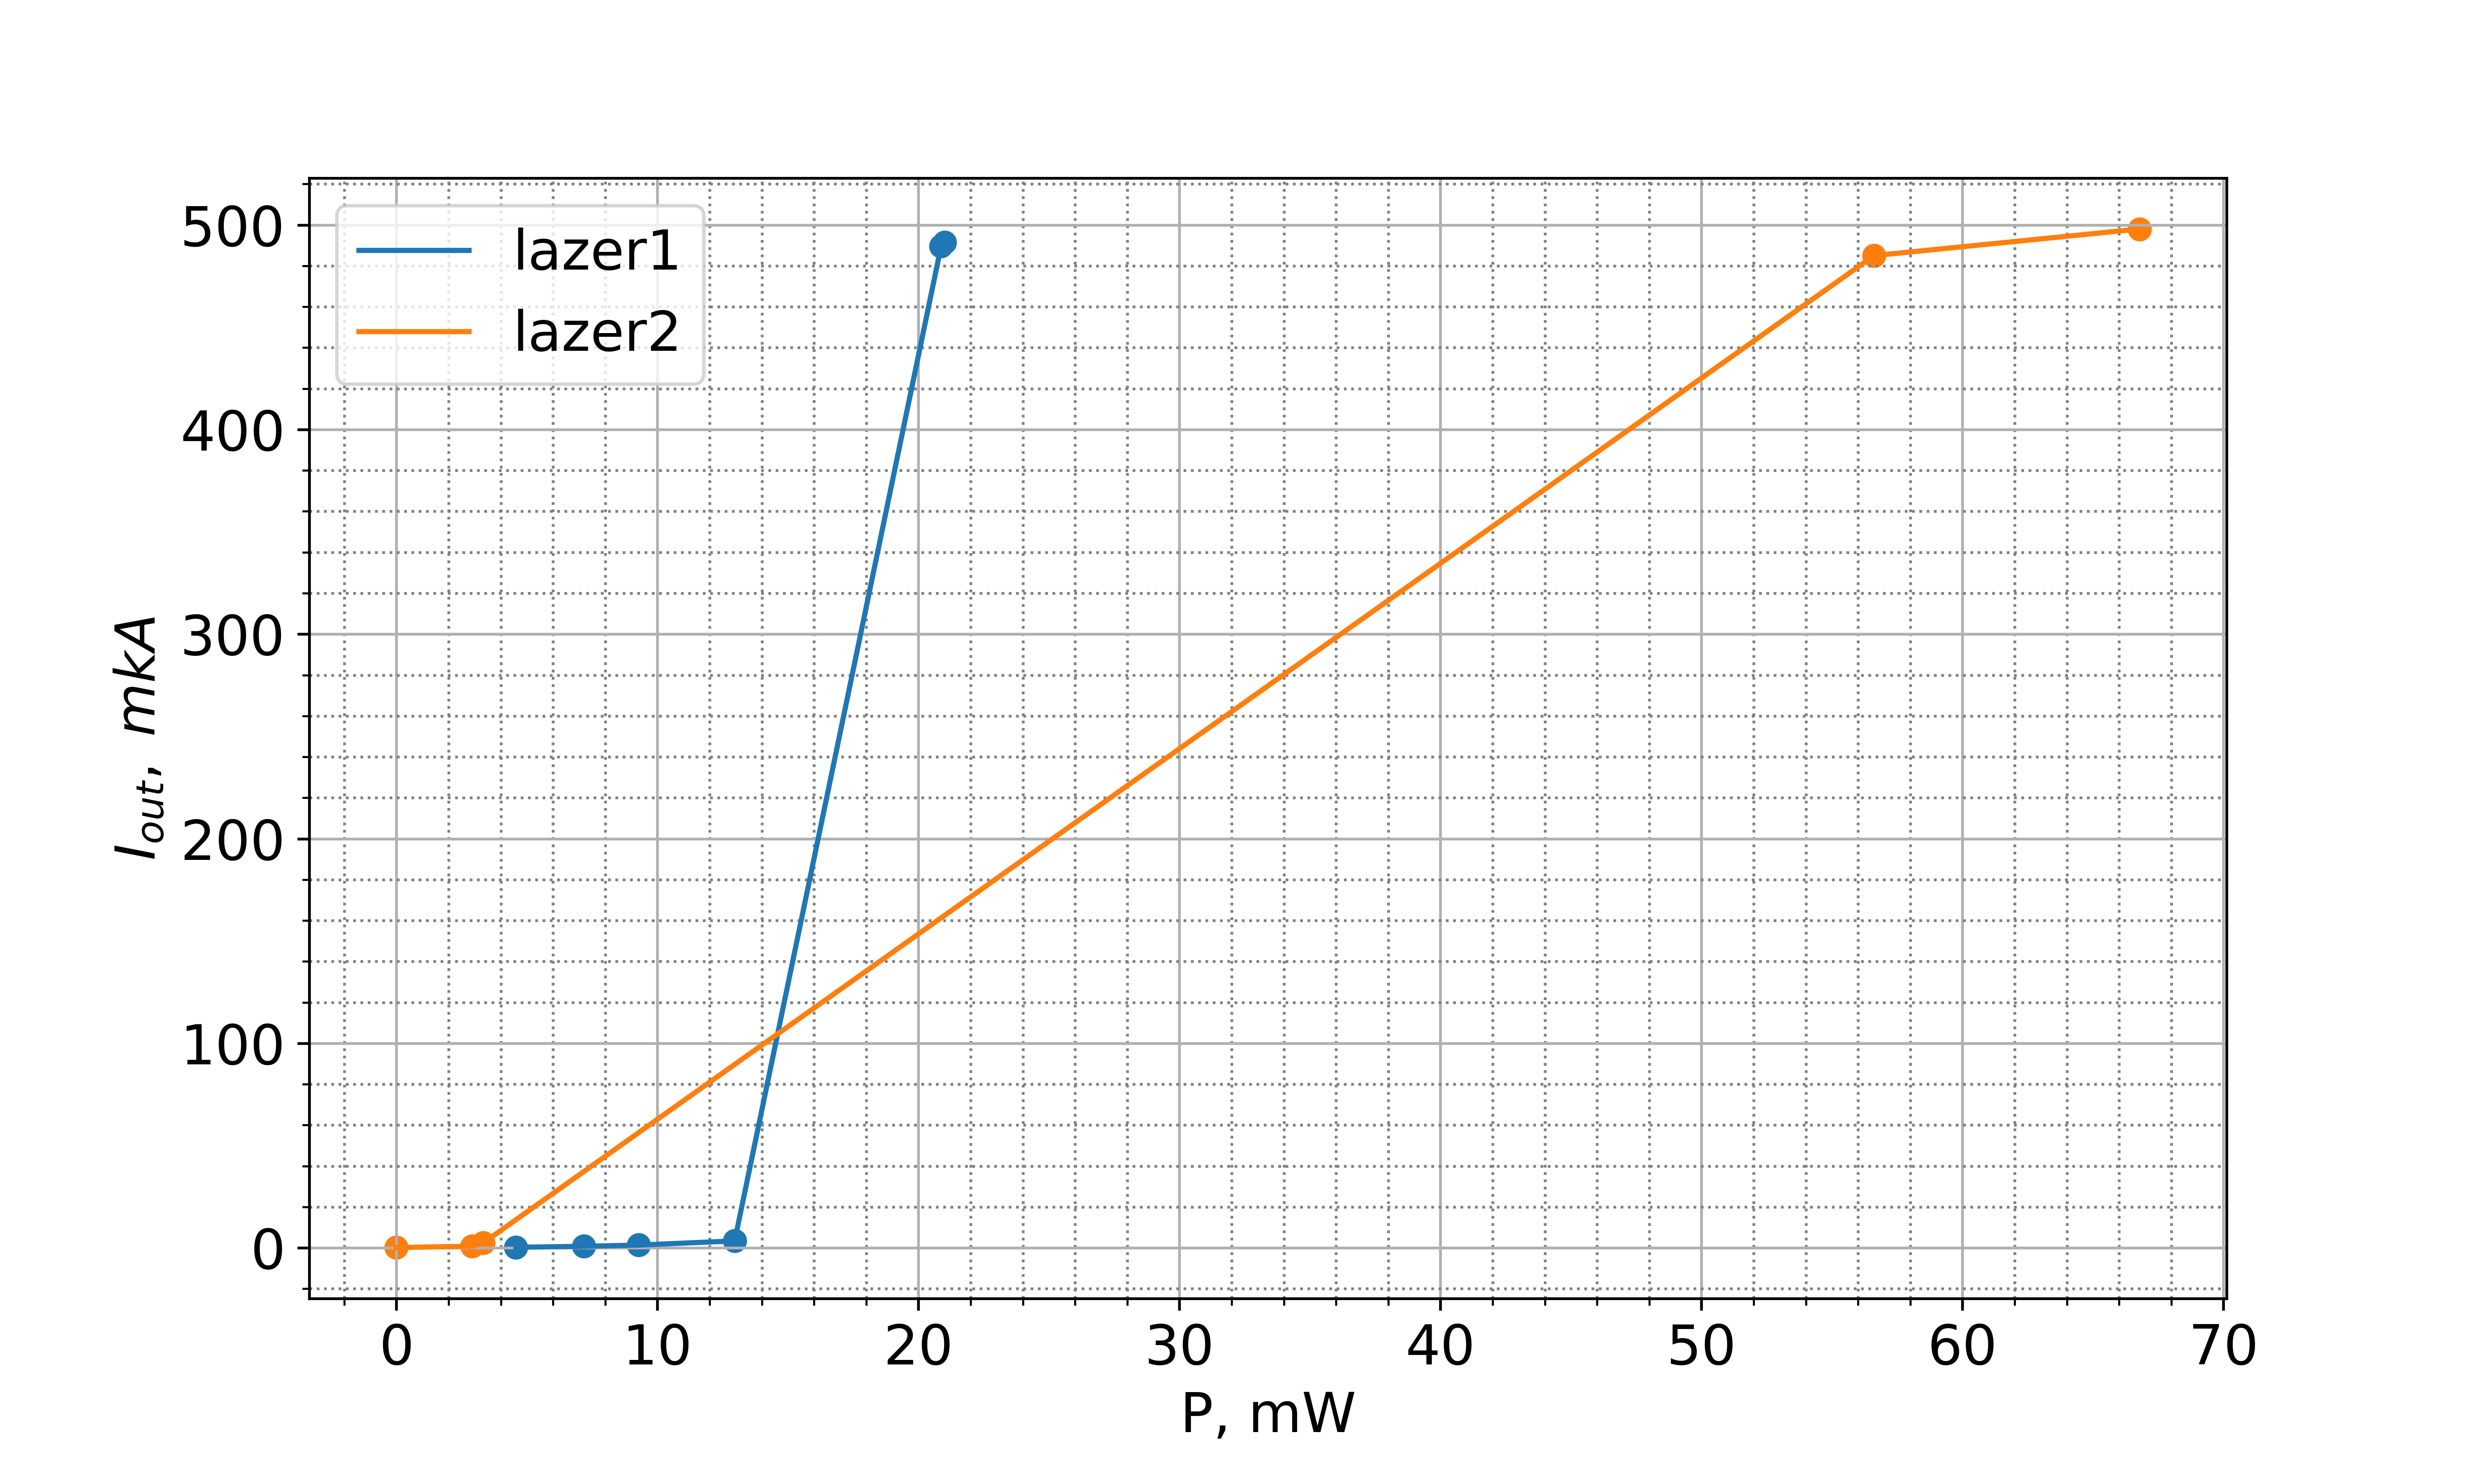
\includegraphics[scale=0.5]{WW-laser.png}
                        \caption{В-В зарактеристика лазеров}
                        \label{W-W-lasers}
                    \end{center}
                \end{figure}
                
                \par На гарфике видим три участка участка: недостаток накачки, линейная зависимость, насыщение. \par 
                Определим характерные значения накачки.

                \begin{itemize}
                    \item Пороговая мощность $P_{\mbox{пор}} \approx \textbf{12}\: \mbox{мВт}$; $\textbf{4}\: \mbox{мВт}$
                    \item Мощность насыщения $P_{\mbox{нас}} \approx \textbf{21} \:  \mbox{мВт}$; $\textbf{60} \:  \mbox{мВт}$
                \end{itemize}
        
            
            \item \textbf{Зависимости амплитуды выходого сигнала от мощности накачки для трёх диодов} \par
            
                \begin{figure}[H]
                    \begin{center}
                        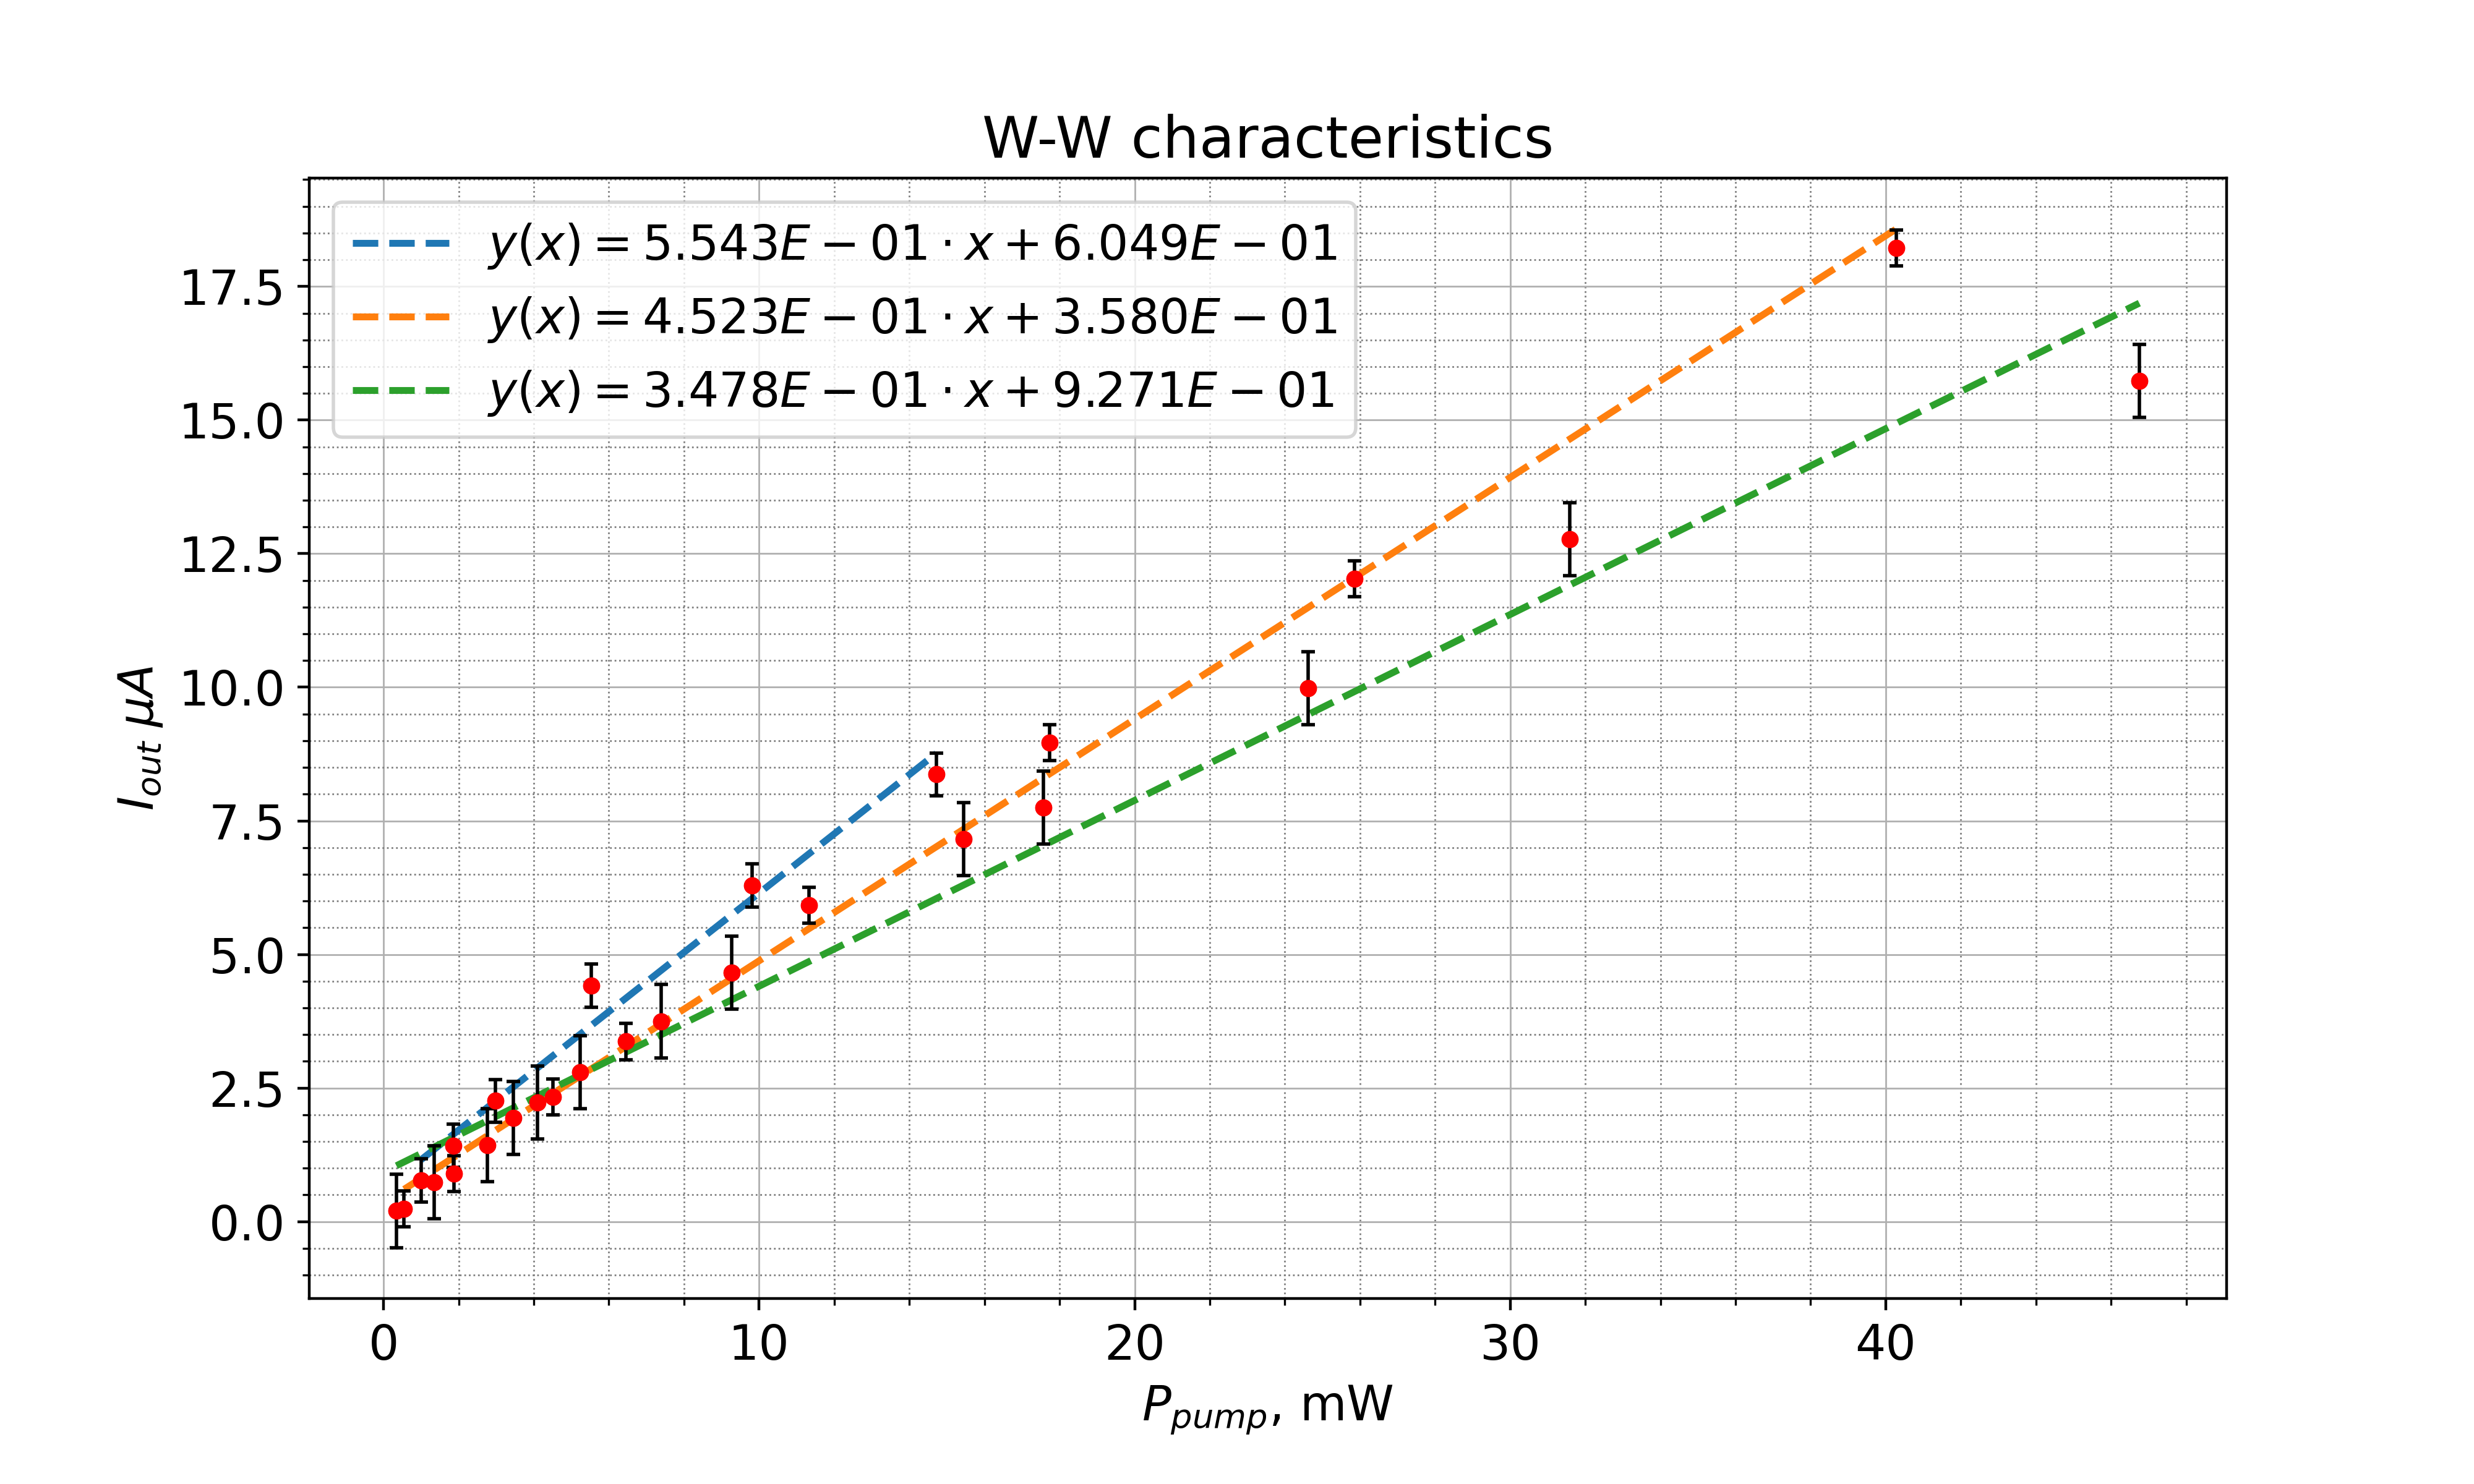
\includegraphics[scale=0.5]{W-W-led.png}
                        \caption{Анимэ на картинке}
                        \label{W-W-led}
                    \end{center}
                \end{figure}
                
                \par В-В характеристика диодов имеет линейный вид, КПД каждого определяется как коэффициент наклона линейного фита, коэффициенты в таблицах (1,2,3)
                
                \begin{table}[H]
\centering
\caption{Коэффициенты аппроксимации Синего диода}
\label{coeffs_table}
\begin{tabular}{lrrr}
\toprule
coeffs &  coeffs\_values &  standard error &  relative se, \% \\
\midrule
   a\_0 &      5.543E-01 &       1.715E-03 &       3.094E-01 \\
   a\_1 &      6.049E-01 &       1.020E-01 &       1.686E+01 \\
\bottomrule
\end{tabular}
\end{table}

                \begin{table}[H]
\centering
\caption{Коэффициенты аппроксимации красного богатыря}
\label{coeffs_table}
\begin{tabular}{lrrr}
\toprule
coeffs &  coeffs\_values &  standard error &  relative se, \% \\
\midrule
   a\_0 &      4.523E-01 &       1.139E-04 &       2.518E-02 \\
   a\_1 &      3.580E-01 &       3.985E-02 &       1.113E+01 \\
\bottomrule
\end{tabular}
\end{table}

                \begin{table}[H]
\centering
\caption{Коэффициенты аппроксимации зеленого диода}
\label{coeffs_table}
\begin{tabular}{lrrr}
\toprule
coeffs &  coeffs\_values &  standard error &  relative se, \% \\
\midrule
   a\_0 &      3.478E-01 &       2.382E-04 &       6.849E-02 \\
   a\_1 &      9.271E-01 &       8.325E-02 &       8.979E+00 \\
\bottomrule
\end{tabular}
\end{table}

        
        \end{enumerate}
    
\section{Выводы}

    \begin{itemize}
        \item Рост мощность накачки увеличивает ширину спектра излучения лазера, не меняя частоту генерации;
        \item Рост мощность накачки увеличивает ширину спектра излучения диода, снижая частоту генерации;
        \item Лазер имеет наименьшую ширину спектра излучения при сравнимых мощностях накачки;
        \item Диоды имеют линейную ватт-ваттную характеристику;
        \item Лазер имеет линейную ВВХ в диапазоне мощностей накачки, от 12 до 21 мВт и от 4 до 60 мВт;
        \item КПД диодов: красный 45\%, зеленый 35\%, синий 55\%;
    \end{itemize}


\end{document}